%%%%%%%%%%%%%%%%%%%%%%%%%%%%%%%%%%%%%%%%%%%%%%%%%%%%%%%%%%%%%%%%%%%%%%%%%%%%%%%%
%%%%%%%%%%%%%%%%%%%%%%%%%%%%%%%%%%%%%%%%%%%%%%%%%%%%%%%%%%%%%%%%%%%%%%%%%%%%%%%%
%%%%%%%%%%%%%%%%%%%%%%%%%%%%%%%%%%%%%%%%%%%%%%%%%%%%%%%%%%%%%%%%%%%%%%%%%%%%%%%%
%%%%%%%%%%%%%%%%%%%%%%%%%%%%%%%%%%%%%%%%%%%%%%%%%%%%%%%%%%%%%%%%%%%%%%%%%%%%%%%%
\chapter{Correction des systèmes asservis\label{chap-correc}}
%%%%%%%%%%%%%%%%%%%%%%%%%%%%%%%%%%%%%%%%%%%%%%%%%%%%%%%%%%%%%%%%%%%%%%%%%%%%%%%%
%%%%%%%%%%%%%%%%%%%%%%%%%%%%%%%%%%%%%%%%%%%%%%%%%%%%%%%%%%%%%%%%%%%%%%%%%%%%%%%%
%%%%%%%%%%%%%%%%%%%%%%%%%%%%%%%%%%%%%%%%%%%%%%%%%%%%%%%%%%%%%%%%%%%%%%%%%%%%%%%%
%%%%%%%%%%%%%%%%%%%%%%%%%%%%%%%%%%%%%%%%%%%%%%%%%%%%%%%%%%%%%%%%%%%%%%%%%%%%%%%%
\minitoc
\newpage
%%%%%%%%%%%%%%%%%%%%%%%%%%%%%%%%%%%%%%%%%%%%%%%%%%%%%%%%%%%%%%%%%%%%%%%%%%%%%%%%
%%%%%%%%%%%%%%%%%%%%%%%%%%%%%%%%%%%%%%%%%%%%%%%%%%%%%%%%%%%%%%%%%%%%%%%%%%%%%%%%
%%%%%%%%%%%%%%%%%%%%%%%%%%%%%%%%%%%%%%%%%%%%%%%%%%%%%%%%%%%%%%%%%%%%%%%%%%%%%%%%
\section{Nécessité de la correction}
%%%%%%%%%%%%%%%%%%%%%%%%%%%%%%%%%%%%%%%%%%%%%%%%%%%%%%%%%%%%%%%%%%%%%%%%%%%%%%%%
%%%%%%%%%%%%%%%%%%%%%%%%%%%%%%%%%%%%%%%%%%%%%%%%%%%%%%%%%%%%%%%%%%%%%%%%%%%%%%%%
%%%%%%%%%%%%%%%%%%%%%%%%%%%%%%%%%%%%%%%%%%%%%%%%%%%%%%%%%%%%%%%%%%%%%%%%%%%%%%%%

%%%%%%%%%%%%%%%%%%%%%%%%%%%%%%%%%%%%%%%%%%%%%%%%%%%%%%%%%%%%%%%%%%%%%%%%%%%%%%%%
%%%%%%%%%%%%%%%%%%%%%%%%%%%%%%%%%%%%%%%%%%%%%%%%%%%%%%%%%%%%%%%%%%%%%%%%%%%%%%%%
%%%%%%%%%%%%%%%%%%%%%%%%%%%%%%%%%%%%%%%%%%%%%%%%%%%%%%%%%%%%%%%%%%%%%%%%%%%%%%%%
\section{Structure de la correction}
%%%%%%%%%%%%%%%%%%%%%%%%%%%%%%%%%%%%%%%%%%%%%%%%%%%%%%%%%%%%%%%%%%%%%%%%%%%%%%%%
%%%%%%%%%%%%%%%%%%%%%%%%%%%%%%%%%%%%%%%%%%%%%%%%%%%%%%%%%%%%%%%%%%%%%%%%%%%%%%%%
%%%%%%%%%%%%%%%%%%%%%%%%%%%%%%%%%%%%%%%%%%%%%%%%%%%%%%%%%%%%%%%%%%%%%%%%%%%%%%%%
\textbf{La correction élabore une commande $u(t)$ à partir d'un écart 
$\epsilon(t)$}
%-------------------------------------------------------------------------------
\begin{center}
    \tikzsetnextfilename{bs_correction_chap_correction-ext}
    \begin{tikzpicture}
    \bs[$\epsilon(p)$][$C(p)$][Correcteur][$U(p)$]
\end{tikzpicture}

\end{center}
%-------------------------------------------------------------------------------
%%%%%%%%%%%%%%%%%%%%%%%%%%%%%%%%%%%%%%%%%%%%%%%%%%%%%%%%%%%%%%%%%%%%%%%%%%%%%%%%
\paragraph{Correcteur série}
%%%%%%%%%%%%%%%%%%%%%%%%%%%%%%%%%%%%%%%%%%%%%%%%%%%%%%%%%%%%%%%%%%%%%%%%%%%%%%%%
%-------------------------------------------------------------------------------
\begin{center}
    \tikzsetnextfilename{correction_serie_chap_correction-ext}
    \begin{tikzpicture}
    \corrbruni
\end{tikzpicture}

\end{center}
%-------------------------------------------------------------------------------
\[
    U(p)=C(p)\epsilon(p)
\]
\[
    H_{BO}(p)=C(p)H(p)
\]
\[
    H_{BF}(p)=\dfrac{C(p)H(p)}{1+C(p)H(p)}
\]
%%%%%%%%%%%%%%%%%%%%%%%%%%%%%%%%%%%%%%%%%%%%%%%%%%%%%%%%%%%%%%%%%%%%%%%%%%%%%%%%
\paragraph{Correcteur en réaction}
%%%%%%%%%%%%%%%%%%%%%%%%%%%%%%%%%%%%%%%%%%%%%%%%%%%%%%%%%%%%%%%%%%%%%%%%%%%%%%%%
%-------------------------------------------------------------------------------
\begin{center}
    \tikzsetnextfilename{correction_reaction_chap_correction-ext}
    \begin{tikzpicture}
    \sbEntree{E1}
    \sbComp[4.5]{comp}{E1}
    \sbRelier[$E(p)$]{E1}{comp}
    \sbComp[4.5]{comp2}{comp}
    \sbRelier[$\epsilon(p)$]{comp}{comp2}
    \sbBloc[3]{B1}{$H(p)$}{comp2}
    \sbRelier[$U(p)$]{comp2}{B1}
    \sbSortie[6]{S1}{B1}
    \sbRelier{B1}{S1}
    \sbNomLien[0.8]{S1}{$S(p)$}
    \sbRenvoi[8]{B1-S1}{comp}{}
    \sbDecaleNoeudy{B1}{R}
    \sbBlocr[-1.75]{R1}{$C(p)$}{R}
    \sbRelieryx{B1-S1}{R1}
    \sbRelierxy{R1}{comp2}
\end{tikzpicture}

\end{center}
%-------------------------------------------------------------------------------
\[
    U(p)=\epsilon(p)-C(p)S(p)
\]
\[
    H_{BO}(p)=\dfrac{H(p)}{1+C(p)H(p)}
\]
\[
    H_{BF}(p)=\dfrac{H(p)}{1+H(p)+C(p)H(p)}
\]
%%%%%%%%%%%%%%%%%%%%%%%%%%%%%%%%%%%%%%%%%%%%%%%%%%%%%%%%%%%%%%%%%%%%%%%%%%%%%%%%
\paragraph{Correcteur en série-réaction}
%%%%%%%%%%%%%%%%%%%%%%%%%%%%%%%%%%%%%%%%%%%%%%%%%%%%%%%%%%%%%%%%%%%%%%%%%%%%%%%%
%-------------------------------------------------------------------------------
\begin{center}
    \tikzsetnextfilename{correction_serie-reaction_chap_correction-ext}
    \input{tikz/correction_serie-reaction_chap_correction.tex}
\end{center}
%-------------------------------------------------------------------------------
\[
    U(p)=C_1(p)\epsilon(p)-C_2(p)S(p)
\]
\[
    H_{BO}(p)=\dfrac{C_1(p)H(p)}{1+C_2(p)H(p)}
\]
\[
    H_{BF}(p)=\dfrac{C_1(p)H(p)}{1+C_1(p)H(p)+C_2(p)H(p)}
\]
%%%%%%%%%%%%%%%%%%%%%%%%%%%%%%%%%%%%%%%%%%%%%%%%%%%%%%%%%%%%%%%%%%%%%%%%%%%%%%%%
%%%%%%%%%%%%%%%%%%%%%%%%%%%%%%%%%%%%%%%%%%%%%%%%%%%%%%%%%%%%%%%%%%%%%%%%%%%%%%%%
%%%%%%%%%%%%%%%%%%%%%%%%%%%%%%%%%%%%%%%%%%%%%%%%%%%%%%%%%%%%%%%%%%%%%%%%%%%%%%%%
\section{Correcteurs élémentaires P, I et D}
%%%%%%%%%%%%%%%%%%%%%%%%%%%%%%%%%%%%%%%%%%%%%%%%%%%%%%%%%%%%%%%%%%%%%%%%%%%%%%%%
%%%%%%%%%%%%%%%%%%%%%%%%%%%%%%%%%%%%%%%%%%%%%%%%%%%%%%%%%%%%%%%%%%%%%%%%%%%%%%%%
%%%%%%%%%%%%%%%%%%%%%%%%%%%%%%%%%%%%%%%%%%%%%%%%%%%%%%%%%%%%%%%%%%%%%%%%%%%%%%%%
%%%%%%%%%%%%%%%%%%%%%%%%%%%%%%%%%%%%%%%%%%%%%%%%%%%%%%%%%%%%%%%%%%%%%%%%%%%%%%%%
%%%%%%%%%%%%%%%%%%%%%%%%%%%%%%%%%%%%%%%%%%%%%%%%%%%%%%%%%%%%%%%%%%%%%%%%%%%%%%%%
\subsection{Correcteur P}
%%%%%%%%%%%%%%%%%%%%%%%%%%%%%%%%%%%%%%%%%%%%%%%%%%%%%%%%%%%%%%%%%%%%%%%%%%%%%%%%
%%%%%%%%%%%%%%%%%%%%%%%%%%%%%%%%%%%%%%%%%%%%%%%%%%%%%%%%%%%%%%%%%%%%%%%%%%%%%%%%
\index{Correcteur ! Proportionnel (P)}
%-------------------------------------------------------------------------------
\begin{center}
    \tikzsetnextfilename{p_chap_correction-ext}
    \begin{tikzpicture}
    \sbStyleBloc{col4}
    \bs[$\epsilon(p)$][$k_p$][][$U(p)$]
\end{tikzpicture}

\end{center}
%-------------------------------------------------------------------------------
%-------------------------------------------------------------------------------
\begin{bequation}[ams align]
    C_{\text{P}}(p)=k_p 
\end{bequation}
%-------------------------------------------------------------------------------
%%%%%%%%%%%%%%%%%%%%%%%%%%%%%%%%%%%%%%%%%%%%%%%%%%%%%%%%%%%%%%%%%%%%%%%%%%%%%%%%
%%%%%%%%%%%%%%%%%%%%%%%%%%%%%%%%%%%%%%%%%%%%%%%%%%%%%%%%%%%%%%%%%%%%%%%%%%%%%%%%
\subsection{Correcteur I}
%%%%%%%%%%%%%%%%%%%%%%%%%%%%%%%%%%%%%%%%%%%%%%%%%%%%%%%%%%%%%%%%%%%%%%%%%%%%%%%%
%%%%%%%%%%%%%%%%%%%%%%%%%%%%%%%%%%%%%%%%%%%%%%%%%%%%%%%%%%%%%%%%%%%%%%%%%%%%%%%%
\index{Correcteur ! Intégral (I)}
%-------------------------------------------------------------------------------
\begin{center}
    \tikzsetnextfilename{i_chap_correction-ext}
    \begin{tikzpicture}
    \sbStyleBloc{col3}
    \bs[$\epsilon(p)$][$\dfrac{1}{\tau_i p}$][][$U(p)$]
\end{tikzpicture}

\end{center}
%-------------------------------------------------------------------------------
%-------------------------------------------------------------------------------
\begin{bequation}[ams align]
    C_{\text{I}}(p)=\dfrac{1}{\tau_i p} 
\end{bequation}
%-------------------------------------------------------------------------------
%%%%%%%%%%%%%%%%%%%%%%%%%%%%%%%%%%%%%%%%%%%%%%%%%%%%%%%%%%%%%%%%%%%%%%%%%%%%%%%%
%%%%%%%%%%%%%%%%%%%%%%%%%%%%%%%%%%%%%%%%%%%%%%%%%%%%%%%%%%%%%%%%%%%%%%%%%%%%%%%%
\subsection{Correcteur D}
%%%%%%%%%%%%%%%%%%%%%%%%%%%%%%%%%%%%%%%%%%%%%%%%%%%%%%%%%%%%%%%%%%%%%%%%%%%%%%%%
%%%%%%%%%%%%%%%%%%%%%%%%%%%%%%%%%%%%%%%%%%%%%%%%%%%%%%%%%%%%%%%%%%%%%%%%%%%%%%%%
\index{Correcteur ! Dérivé (D)}
%-------------------------------------------------------------------------------
\begin{center}
    \tikzsetnextfilename{d_chap_correction-ext}
    \begin{tikzpicture}
    \sbStyleBloc{col1}
    \bs[$\epsilon(p)$][$\tau_d p$][][$U(p)$]
\end{tikzpicture}

\end{center}
%-------------------------------------------------------------------------------
%-------------------------------------------------------------------------------
\begin{bequation}[ams align]
    C_{\text{D}}^{\text{idéal}}(p)=\tau_d p 
\end{bequation}
%-------------------------------------------------------------------------------
Le correcteur dérivé sous cette forme est purement théorique, notamment parce
que le gain est infini lorsque la pulsation tend vers l'infini.

Une solution technologique permet de réaliser une forme approché :
\[
    C_{\text{D}}^{\text{réel}}(p)=\dfrac{\tau_d p}{1+\tau p}
\]
en choissisant un temps $\tau\ll\tau_d$, cette fonction de transfert se comporte
comme un correcteur dérivé idéal.
%%%%%%%%%%%%%%%%%%%%%%%%%%%%%%%%%%%%%%%%%%%%%%%%%%%%%%%%%%%%%%%%%%%%%%%%%%%%%%%%
%%%%%%%%%%%%%%%%%%%%%%%%%%%%%%%%%%%%%%%%%%%%%%%%%%%%%%%%%%%%%%%%%%%%%%%%%%%%%%%%
%%%%%%%%%%%%%%%%%%%%%%%%%%%%%%%%%%%%%%%%%%%%%%%%%%%%%%%%%%%%%%%%%%%%%%%%%%%%%%%%
\section{Correcteurs composés}
%%%%%%%%%%%%%%%%%%%%%%%%%%%%%%%%%%%%%%%%%%%%%%%%%%%%%%%%%%%%%%%%%%%%%%%%%%%%%%%%
%%%%%%%%%%%%%%%%%%%%%%%%%%%%%%%%%%%%%%%%%%%%%%%%%%%%%%%%%%%%%%%%%%%%%%%%%%%%%%%%
%%%%%%%%%%%%%%%%%%%%%%%%%%%%%%%%%%%%%%%%%%%%%%%%%%%%%%%%%%%%%%%%%%%%%%%%%%%%%%%%
Comme leurs noms l'indique, les correcteurs composés combinent plusieurs
des correcteurs élémentaires présentés précedemment.
%%%%%%%%%%%%%%%%%%%%%%%%%%%%%%%%%%%%%%%%%%%%%%%%%%%%%%%%%%%%%%%%%%%%%%%%%%%%%%%%
%%%%%%%%%%%%%%%%%%%%%%%%%%%%%%%%%%%%%%%%%%%%%%%%%%%%%%%%%%%%%%%%%%%%%%%%%%%%%%%%
\subsection{Correcteur PI}
%%%%%%%%%%%%%%%%%%%%%%%%%%%%%%%%%%%%%%%%%%%%%%%%%%%%%%%%%%%%%%%%%%%%%%%%%%%%%%%%
%%%%%%%%%%%%%%%%%%%%%%%%%%%%%%%%%%%%%%%%%%%%%%%%%%%%%%%%%%%%%%%%%%%%%%%%%%%%%%%%
\index{Correcteur ! Proportionnel Intégral (PI)}
%-------------------------------------------------------------------------------
\begin{figure}
    \centering
    \tikzsetnextfilename{bode_pi_gain_chap_correction-ext}
    \input{tikz/bode_pi_gain_chap_correction.tex}
    
    \tikzsetnextfilename{bode_pi_phase_chap_correction-ext}
    \input{tikz/bode_pi_phase_chap_correction.tex}
    \caption{Diagramme de Bode du correcteur à effet proportionnel et intégral.}
\end{figure}
%-------------------------------------------------------------------------------
%-------------------------------------------------------------------------------
\begin{center}
    \tikzsetnextfilename{pi_chap_correction-ext}
     \begin{tikzpicture}
    \sbEntree{E1}
    \sbStyleBloc{col4}
    \sbBloc[3]{B1}{$k_p$}{E1}
    \sbRelier[$\epsilon(p)$]{E1}{B1}
    \sbStyleBloc{col3}
    \sbBloc[3]{B2}{$\dfrac{1}{\tau_i p}$}{B1}
    \sbRelier{B1}{B2}
    \sbCompSum[5]{C1}{B2}{+}{}{+}{ }
    \sbRelier{B2}{C1}
    \sbStyleBloc{col1}
    \sbSortie[3]{S1}{C1}
    \sbRelier[$U(p)$]{C1}{S1}
    \sbRenvoi[-4]{B1-B2}{C1}{}
    \node at ($(B1)+(0.88,0.7)$) {\textcolor{col4}{P}};
    \node at ($(B2)+(0.88,0.7)$) {\textcolor{col3}{I}};
\end{tikzpicture}

\end{center}
%-------------------------------------------------------------------------------
\[
    U(p)=k_p\left(1+\dfrac{1}{\tau_i p}\right)\epsilon(p)
\]
%-------------------------------------------------------------------------------
\begin{bequation}[ams align]
    C_{\text{PI}}=k_p\left(\dfrac{1+\tau_i p}{\tau_i p}\right)
\end{bequation}
%-------------------------------------------------------------------------------
%%%%%%%%%%%%%%%%%%%%%%%%%%%%%%%%%%%%%%%%%%%%%%%%%%%%%%%%%%%%%%%%%%%%%%%%%%%%%%%%
%%%%%%%%%%%%%%%%%%%%%%%%%%%%%%%%%%%%%%%%%%%%%%%%%%%%%%%%%%%%%%%%%%%%%%%%%%%%%%%%
\subsection{Correcteur PD}
%%%%%%%%%%%%%%%%%%%%%%%%%%%%%%%%%%%%%%%%%%%%%%%%%%%%%%%%%%%%%%%%%%%%%%%%%%%%%%%%
%%%%%%%%%%%%%%%%%%%%%%%%%%%%%%%%%%%%%%%%%%%%%%%%%%%%%%%%%%%%%%%%%%%%%%%%%%%%%%%%
\index{Correcteur ! Proportionnel Dérivé (PD)}
%-------------------------------------------------------------------------------
\begin{figure}
    \centering
    \tikzsetnextfilename{bode_pd_gain_chap_correction-ext}
    \begin{tikzpicture}[trim axis left]
    \begin{axis}[
    ticklabel style = {font=\footnotesize},
    width=0.9\textwidth,
    height=0.25\textheight,
    ylabel={Gain (\si{\decibel})},
    xtick={1e-4,1e-3,1e-2,1e-1,1,1e1,1e2,1e3,1e4,1e5},
    ytick={0,10,20,30,40},
    xticklabels={$10^{-4}$,$10^{-3}$,$10^{-2}$,$10^{-1}$,
                 $10^{0}$,$10^{1}$,$10^{2}$,$10^{3}$,$10^{4}$,$10^{5}$},
    yticklabels={0,10,20,30,40},
    xmode=log,ymode=normal,
    xmin=1e-2, xmax=1e2,
    ymin=0, ymax=30,
    grid=both,
    major grid style={black!40},
]
    \pgfmathsetmacro{\td}{1.000001} 
    \pgfmathsetmacro{\wtd}{(1/\td)} 
    \pgfmathsetmacro{\tau}{0.1} 
    \pgfmathsetmacro{\wt}{1.0/\tau} 
    \addplot[ultra thick, col3,domain=1e-2:1e2, samples=201]    
            {10*log10(1+\td*\td*x*x)-10*log10(1+\tau*\tau*x*x)};
    \addplot[ultra thick,col1,domain=1e-2:1e2, samples=201]    
            {10*log10(1+\td*\td*x*x)};
    \addplot[line width=2pt,col4,dashed,domain=\wtd:1e2, samples=51] 
            {20*log10(x)};
    \addplot[line width=2pt,col4,dashed,domain=1e-2:\wtd, samples=51] {0};
\end{axis}
\end{tikzpicture}

    
    \tikzsetnextfilename{bode_pd_phase_chap_correction-ext}
    \begin{tikzpicture}[trim axis left]
\begin{axis}[
    ticklabel style = {font=\footnotesize},
    width=0.9\textwidth,
    height=0.25\textheight,
    xlabel={Pulsation (\si{\radian\per\second})},
    ylabel={Phase (\degreeSI)},
    xtick={1e-4,1e-3,1e-2,1e-1,1,1e1,1e2,1e3,1e4,1e5},
    ytick={0,15,30,45,60,75,90},
    yticklabels={0,,30,,60,,90},
    xticklabels={$10^{-4}$,$10^{-3}$,$10^{-2}$,$10^{-1}$,$10^{0}$,
                 $10^{1}$,$10^{2}$,$10^{3}$,$10^{4}$,$10^{5}$},
    xmode=log,ymode=normal,
    xmin=1e-2, xmax=1e2,
    ymin=0, ymax=90,
    grid=both,
    major grid style={black!40},
    %clip=false
]
    \pgfmathsetmacro{\td}{1.0} 
    \pgfmathsetmacro{\wtd}{1.0/\td} 
    \pgfmathsetmacro{\tau}{0.1} 
    \pgfmathsetmacro{\wt}{1.0/\tau} 
    \addplot[ultra thick, col1,domain=1e-2:1e2, samples=201] 
    {atan2(\td*x,1)};
    \addplot[ultra thick, col3,domain=1e-2:1e2, samples=201] 
    {atan2(\td*x,1)-atan2(\tau*x,1)};
    \addplot[line width=2pt,col4,dashed,domain=1e-2:\wtd, samples=51] {0};
    \addplot[line width=2pt,col4,dashed,domain=\wtd:1e2, samples=51] {90};
    \draw[line width=2pt,col4,dashed] 
         (axis cs:\wtd,0) -- (axis cs:\wtd,90);
\end{axis}
\end{tikzpicture}

    \caption{Diagramme de Bode du correcteur à effet proportionnel et dérivé.}
\end{figure}
%-------------------------------------------------------------------------------
%-------------------------------------------------------------------------------
\begin{center}
    \tikzsetnextfilename{pd_chap_correction-ext}
    \begin{tikzpicture}
    \sbEntree{E1}
    \sbStyleBloc{col4}
    \sbBloc[3]{B1}{$k_p$}{E1}
    \sbRelier[$\epsilon(p)$]{E1}{B1}
    \sbStyleBloc{col1}
    \sbBloc[3]{B3}{$\tau_d p$}{B1}
    \sbRelier{B1}{B3}
    \sbCompSum[5]{C2}{B3}{+}{}{+}{ }
    \sbRelier{B3}{C2}
    \sbSortie[3]{S1}{C2}
    \sbRelier[$U(p)$]{C2}{S1}
    \sbRelier{C2}{S1}
    \sbRenvoi[-4]{B1-B3}{C2}{}
    \node at ($(B1)+(0.88,0.7)$) {\textcolor{col4}{P}};
    \node at ($(B3)+(0.88,0.7)$) {\textcolor{col1}{D}};
\end{tikzpicture}

\end{center}
%-------------------------------------------------------------------------------
\[
    U(p)=k_p\left(1+\dfrac{1}{\tau_i p}\right)\epsilon(p)
\]
%-------------------------------------------------------------------------------
\begin{bequation}[ams align]
    C_{\text{PD}}=k_p\left(1+\tau_d p\right)
\end{bequation}
%-------------------------------------------------------------------------------
À l'instar du correcteur dérivé élémentaire, la forme composée PI présente
une forme réel:
\[
    C_{\text{PD}}=k_p\dfrac{1+\tau_d p}{1+\tau p}
\]
avec $\tau\ll\tau_d$
%%%%%%%%%%%%%%%%%%%%%%%%%%%%%%%%%%%%%%%%%%%%%%%%%%%%%%%%%%%%%%%%%%%%%%%%%%%%%%%%
%%%%%%%%%%%%%%%%%%%%%%%%%%%%%%%%%%%%%%%%%%%%%%%%%%%%%%%%%%%%%%%%%%%%%%%%%%%%%%%%
%%%%%%%%%%%%%%%%%%%%%%%%%%%%%%%%%%%%%%%%%%%%%%%%%%%%%%%%%%%%%%%%%%%%%%%%%%%%%%%%
\section{Correcteur à avance et retard de phase}
%%%%%%%%%%%%%%%%%%%%%%%%%%%%%%%%%%%%%%%%%%%%%%%%%%%%%%%%%%%%%%%%%%%%%%%%%%%%%%%%
%%%%%%%%%%%%%%%%%%%%%%%%%%%%%%%%%%%%%%%%%%%%%%%%%%%%%%%%%%%%%%%%%%%%%%%%%%%%%%%%
%%%%%%%%%%%%%%%%%%%%%%%%%%%%%%%%%%%%%%%%%%%%%%%%%%%%%%%%%%%%%%%%%%%%%%%%%%%%%%%%
%%%%%%%%%%%%%%%%%%%%%%%%%%%%%%%%%%%%%%%%%%%%%%%%%%%%%%%%%%%%%%%%%%%%%%%%%%%%%%%%
%%%%%%%%%%%%%%%%%%%%%%%%%%%%%%%%%%%%%%%%%%%%%%%%%%%%%%%%%%%%%%%%%%%%%%%%%%%%%%%%
\subsection{Correcteur à avance de phase}
%%%%%%%%%%%%%%%%%%%%%%%%%%%%%%%%%%%%%%%%%%%%%%%%%%%%%%%%%%%%%%%%%%%%%%%%%%%%%%%%
%%%%%%%%%%%%%%%%%%%%%%%%%%%%%%%%%%%%%%%%%%%%%%%%%%%%%%%%%%%%%%%%%%%%%%%%%%%%%%%%
\index{Correcteur ! à avance de phase (AP)}
Le correcteur à avance de phase (AP) est défini par la fonction de transfert :
%-------------------------------------------------------------------------------
\begin{bequation}[ams align]
    C_{\text{AP}}(p)=k_p\dfrac{1+\alpha\tau p}{1+\tau p} 
\end{bequation}
%-------------------------------------------------------------------------------
avec $\alpha>1$.
%-------------------------------------------------------------------------------
\begin{figure}
    \centering
    \tikzsetnextfilename{bode_avancedephase_gain_chap_correction-ext}
    \begin{tikzpicture}[trim axis left]
    \begin{axis}[
    ticklabel style = {font=\footnotesize},
    width=0.9\textwidth,
    height=0.25\textheight,
    ylabel={Gain (\si{\decibel})},
    xtick={1e-4,1e-3,1e-2,1e-1,1,1e1,1e2,1e3,1e4,1e5},
    ytick={0,1,2,3,4,5,6,7,8,9,10,11,12,13,14,15},
    xticklabels={$10^{-4}$,$10^{-3}$,$10^{-2}$,$10^{-1}$,
                 $10^{0}$,$10^{1}$,$10^{2}$,$10^{3}$,$10^{4}$,$10^{5}$},
    yticklabels={0,,2,,4,,6,,8,,10,,12,,14},
    xmode=log,ymode=normal,
    xmin=1e-2, xmax=1e2,
    ymin=0, ymax=15,
    grid=both,
    major grid style={black!40},
    clip=false,
]
    \pgfmathsetmacro{\aa}{5.001} 
    \pgfmathsetmacro{\ia}{(1/\aa)} 
    \pgfmathsetmacro{\wm}{(1/sqrt(\aa))} 
    \pgfmathsetmacro{\gm}{10*log10(\aa)} 
    \pgfmathsetmacro{\dgm}{20*log10(\aa)} 
    \addplot[ultra thick, col1,domain=1e-2:1e2, samples=201]    
            {10*log10(1+\aa*\aa*x*x)-10*log10(1+x*x)};
    \addplot[line width=2pt,col4,dashed,domain=1e0:1e2, samples=51] 
            {20*log10(\aa)};
    \addplot[line width=2pt,col4,dashed,domain=1e-2:\ia, samples=51] {0};
    \addplot[line width=2pt,col4,dashed,domain=\ia:1e0, samples=101] 
            {20*log10(\aa)+20*log10(x)};
    \draw[line width=2pt,col2,-latex] 
         (axis cs:\wm,0) node[below] {$\omega_m$}  -- 
         node[right] {$\boldsymbol{10\log{\alpha}}$} (axis cs:\wm,\gm);
    \draw[line width=2pt,col2,-latex] 
        (axis cs:10,0)  --
        node[right] {$\boldsymbol{20\log{\alpha}}$} (axis cs:10,\dgm);
\end{axis}
\end{tikzpicture}


    
    \tikzsetnextfilename{bode_avancedephase_phase_chap_correction-ext}
    \input{tikz/bode_avancedephase_phase_chap_correction.tex}
    \caption{Diagramme de Bode du correcteur à avance de phase.}
\end{figure}
%-------------------------------------------------------------------------------
Le maximum de la phase se trouve à la moyenne géométrique du segment 
$\left[\dfrac{1}{\alpha\tau},\dfrac{1}{\alpha}\right]$ (l'echelle étant 
logarithmique ceux sont les rapports qui sont égaux)
\[
    \omega_m^2=\dfrac{1}{\alpha\tau^2}
\]
ou encore 
\[
    \omega_m=\dfrac{1}{\sqrt{\alpha}\tau}
\]
Pour $k_p=1$, $\alpha=5$ et $\tau=1$ on a alors 
$\omega_m=\SI{1}{\sqrt{5}}\sim\SI{0.44}{\radian\per\second}$.
\[
    \phi(\omega)=\arg{(C_{\text{AP}}(\jw))}
                =\arctan{\alpha\tau\omega_m}-\arctan{\tau\omega_m}
\]

\[
    \phi_m=\phi(\omega_m)=\arctan{\alpha\tau\omega_m}-\arctan{\tau\omega_m}
\]
en utilisant la relation trigonométrique pour $\tan{(a-b)}$ et en posant 
$a=\arctan{\alpha\tau\omega_m}$ et $b=\arctan{\tau\omega_m}$, on écrit:
\[
    \tan{\phi(\omega_m)}=\dfrac{\alpha\tau\omega_m-\tau\omega_m}
                               {1+\alpha\tau^2\omega_m^2}
                        =\dfrac{\alpha-1}{2\sqrt{\alpha}}
\]
donc on a :
\[
    \phi_m=\arctan{\left(\dfrac{\alpha-1}{2\sqrt{\alpha}}\right)}
\]
Une autre forme possible est également donnée par 
(en notant que $\sin\arctan{x}=\dfrac{x}{\sqrt{1+x^2}}$):
\[
    \phi_m=\arcsin{\left(\dfrac{\alpha-1}{\alpha+1}\right)}
\]
On remarquera que le maximum ne dépend pas de $\tau$.
Pour $\alpha=5$, $\phi_m=\SI{41.8}{\degree}$.

Le gain pour la pulsation $\omega_m$ est donné par:
\[
    C_{\text{AP},\si{\dB}}(j\omega_m)=10\log{(1+\alpha^2\tau^2\omega_m^2)}-
                               10\log{(1+\tau^2\omega_m^2)}
\]
puisque $\tau^2\omega_m^2=\dfrac{1}{\alpha}$.
\[
    C_{\text{AP},\si{\dB}}(j\omega_m)=
    10\log{1+\alpha}-10\log{\dfrac{1+\alpha}{\alpha}}=10\log{\alpha}
\]
%%%%%%%%%%%%%%%%%%%%%%%%%%%%%%%%%%%%%%%%%%%%%%%%%%%%%%%%%%%%%%%%%%%%%%%%%%%%%%%%
%%%%%%%%%%%%%%%%%%%%%%%%%%%%%%%%%%%%%%%%%%%%%%%%%%%%%%%%%%%%%%%%%%%%%%%%%%%%%%%%
\subsection{Correcteur à retard de phase}
%%%%%%%%%%%%%%%%%%%%%%%%%%%%%%%%%%%%%%%%%%%%%%%%%%%%%%%%%%%%%%%%%%%%%%%%%%%%%%%%
%%%%%%%%%%%%%%%%%%%%%%%%%%%%%%%%%%%%%%%%%%%%%%%%%%%%%%%%%%%%%%%%%%%%%%%%%%%%%%%%
\index{Correcteur ! à retard de phase (RP)}
Le correcteur à retard de phase (RP) est défini par la fonction de transfert :
%-------------------------------------------------------------------------------
\begin{bequation}[ams align]
    C_{\text{RP}}(p)=k_p\dfrac{1+\tau p}{1+\beta\tau p}
\end{bequation}
%-------------------------------------------------------------------------------
avec $\beta>1$
%-------------------------------------------------------------------------------
\begin{figure}
    \centering
    \tikzsetnextfilename{bode_retarddephase_gain_chap_correction-ext}
    \begin{tikzpicture}[trim axis left]
\begin{axis}[
    ticklabel style = {font=\footnotesize},
    width=0.9\textwidth,
    height=0.25\textheight,
    ylabel={Gain (\si{\decibel})},
    xtick={1e-4,1e-3,1e-2,1e-1,1,1e1,1e2,1e3,1e4,1e5},
    ytick={-15,-14,-13,-12,-11,-10,-9,-8,-7,-6,-5,-4,-3,-2,-1,0},
    xticklabels={$10^{-4}$,$10^{-3}$,$10^{-2}$,$10^{-1}$,
                 $10^{0}$,$10^{1}$,$10^{2}$,$10^{3}$,$10^{4}$,$10^{5}$},
    yticklabels={,-14,,-12,,-10,,-8,,-6,,-4,,-2,,0},
    xmode=log,ymode=normal,
    xmin=1e-2, xmax=1e2,
    ymin=-15, ymax=0,
    grid=both,
    major grid style={black!40},
    clip=false,
]
    \pgfmathsetmacro{\bb}{5.0} 
    \pgfmathsetmacro{\ib}{(1/\bb)} 
    \pgfmathsetmacro{\wm}{(1/sqrt(\bb))} 
    \pgfmathsetmacro{\gm}{10*log10(\bb)} 
    \pgfmathsetmacro{\dgm}{20*log10(\bb)} 
    \addplot[ultra thick, col1,domain=1e-2:1e2, samples=201] 
    {10*log10(1+x*x)-10*log10(1+\bb*\bb*x*x)};
    \addplot[line width=2pt,col4,dashed,domain=1e-2:\ib, samples=51] {0};
    \addplot[line width=2pt,col4,dashed,domain=\ib:1e0, samples=101] 
    {-20*log10(\bb)-20*log10(x)};
    \addplot[line width=2pt,col4,dashed,domain=1e0:1e2, samples=51] 
    {-20*log10(\bb)};
    \draw[line width=2pt,col2,-latex] 
    (axis cs:\wm,0) node[above] {$\omega_m$}  -- 
    node[right] {$\boldsymbol{10\log{\alpha}}$} (axis cs:\wm,-\gm);
    \draw[line width=2pt,col2,-latex] 
    (axis cs:10,0)  -- node[right] {$\boldsymbol{20\log{\alpha}}$} 
    (axis cs:10,-\dgm);
\end{axis}
\end{tikzpicture}

    
    \tikzsetnextfilename{bode_retarddephase_phase_chap_correction-ext}
    \input{tikz/bode_retarddephase_phase_chap_correction.tex}
    \caption{Diagramme de Bode du correcteur à retard de phase}
\end{figure}
%-------------------------------------------------------------------------------
Le minimum de la phase se trouve à la moyenne géométrique du segment 
$\left[\dfrac{1}{\beta\tau},\dfrac{1}{\tau}\right]$. Cette pulsation 
est donnée par :
\[
    \omega_m=\dfrac{1}{\sqrt{\beta}\tau}
\]
Pour $k_p=1$, $\beta=5$ et $\tau=1$ on a alors 
$\omega_m=\SI{1}{\sqrt{5}}\sim\SI{0.44}{\radian\per\second}$.
\[
    \phi(\omega)=\arg{(C_{\text{RP}}(\jw))}
                =\arctan{\tau\omega_m}-\arctan{\beta\tau\omega_m}
\]

\[
    \phi_m=\phi(\omega_m)=\arctan{\tau\omega_m}-\arctan{\beta\tau\omega_m}
\]
en utilisant la relation trigonométrique pour $\tan{(a-b)}$ et 
en posant $a=\arctan{\tau\omega_m}$ et $b=\arctan{\beta\tau\omega_m}$, 
on écrit:
\[
    \tan{\phi(\omega_m)}=\dfrac{\tau\omega_m-\beta\tau\omega_m}
                               {1+\beta\tau^2\omega_m^2}
                        =\dfrac{1-\beta}{2\sqrt{\beta}}
\]
donc on a :
\[
    \phi_m=\arctan{\left(\dfrac{1-\beta}{2\sqrt{\beta}}\right)}
\]
On remarquera que le maximum ne dépend pas de $\tau$.
Pour $\beta=5$, $\phi_m=\SI{-41.8}{\degree}$.

Le gain pour la pulsation $\omega_m$ est donné par:
\[
    C_{\text{RP},\si{\dB}}(j\omega_m)=10\log{(1+\tau^2\omega_m^2)}-
                               10\log{(1+\beta^2\tau^2\omega_m^2)}
\]
puisque $\tau^2\omega_m^2=\dfrac{1}{\beta}$.
\[
    C_{\text{RP},\si{\dB}}(j\omega_m)=10\log{\left(\dfrac{1+\beta}{\beta}\right)}
                              -10\log{\left(1+\beta\right)}=-10\log{\beta}
\]
%%%%%%%%%%%%%%%%%%%%%%%%%%%%%%%%%%%%%%%%%%%%%%%%%%%%%%%%%%%%%%%%%%%%%%%%%%%%%%%%
%%%%%%%%%%%%%%%%%%%%%%%%%%%%%%%%%%%%%%%%%%%%%%%%%%%%%%%%%%%%%%%%%%%%%%%%%%%%%%%%
\subsection{Correcteur à retard-avance de phase}
%%%%%%%%%%%%%%%%%%%%%%%%%%%%%%%%%%%%%%%%%%%%%%%%%%%%%%%%%%%%%%%%%%%%%%%%%%%%%%%%
%%%%%%%%%%%%%%%%%%%%%%%%%%%%%%%%%%%%%%%%%%%%%%%%%%%%%%%%%%%%%%%%%%%%%%%%%%%%%%%%
\index{Correcteur ! à retard-avance de phase}
Le correcteur à retard-avance de phase (RAP) est défini par la fonction 
de transfert :
%-------------------------------------------------------------------------------
\begin{bequation}[ams align]
    C_{\text{RAP}}(p)=\dfrac{1+\tau_r p}{1+\beta\tau_r p}\cdot
               \dfrac{1+\alpha\tau_a p}{1+\tau_a p}
\end{bequation}
%-------------------------------------------------------------------------------
avec $\alpha>1$ et $\beta>1$. On prendra $\alpha=\beta$.
%-------------------------------------------------------------------------------
\begin{figure}
    \centering
    \tikzsetnextfilename{bode_retardavancedephase_gain_chap_correction-ext}
    \begin{tikzpicture}[trim axis left]
\begin{axis}[
    ticklabel style = {font=\footnotesize},
    width=0.9\textwidth,
    height=0.25\textheight,
    ylabel={Gain (\si{\decibel})},
    xtick={1e-4,1e-3,1e-2,1e-1,1,1e1,1e2,1e3,1e4,1e5},
    ytick={-20,-18,-16,-14,-12,-10,-8,-6,-4,-2,0},
    xticklabels={$10^{-4}$,$10^{-3}$,$10^{-2}$,$10^{-1}$,
                 $10^{0}$,$10^{1}$,$10^{2}$,$10^{3}$,$10^{4}$,$10^{5}$},
    yticklabels={-20,,-16,,-12,,-8,,-4,,0},
    xmode=log,ymode=normal,
    xmin=1e-2, xmax=1e3,
    ymin=-20, ymax=0,
    grid=both,
    major grid style={black!40},
    clip=false,
]
    \pgfmathsetmacro{\ta}{0.02} 
    \pgfmathsetmacro{\tb}{0.25} 
    \pgfmathsetmacro{\aa}{5} 
    \pgfmathsetmacro{\bb}{5} 
    \pgfmathsetmacro{\ib}{(1/(\bb*\tb))} 
    \pgfmathsetmacro{\ia}{(1/(\aa*\ta))} 
    \pgfmathsetmacro{\itb}{(1/\tb)} 
    \pgfmathsetmacro{\ita}{(1/\ta)} 
    \pgfmathsetmacro{\wm}{(1/sqrt(\bb))} 
    \pgfmathsetmacro{\gm}{10*log10(\bb)} 
    \pgfmathsetmacro{\dgm}{20*log10(\bb)} 
    \addplot[ultra thick, col1,domain=1e-2:1e3, samples=201] 
    {10*log10(1+\tb*\tb*x*x)+
     10*log10(1+\aa*\aa*\ta*\ta*x*x)-    
     10*log10(1+\tb*\tb*\bb*\bb*x*x)-
     10*log10(1+\ta*\ta*x*x)};
    \addplot[line width=2pt,col4,dashed,domain=1e-2:\ib, samples=51] {0};
    \addplot[line width=2pt,col4,dashed,domain=\ib:\itb, samples=101] 
    {-20*log10(\bb*\tb)-20*log10(x)};
    \addplot[line width=2pt,col4,dashed,domain=\itb:\ia, samples=51] 
    {-20*log10(\bb)};
    \addplot[line width=2pt,col4,dashed,domain=\ia:\ita, samples=51] 
    {20*log10(\ta)+20*log10(x)};
    \addplot[line width=2pt,col4,dashed,domain=\ita:1e3, samples=51] {0};
\end{axis}
\end{tikzpicture}

    
    \tikzsetnextfilename{bode_retardavancedephase_phase_chap_correction-ext}
    \begin{tikzpicture}[trim axis left]
\begin{axis}[
    ticklabel style = {font=\footnotesize},
    width=0.9\textwidth,
    height=0.25\textheight,
    xlabel={Pulsation (\si{\radian\per\second})},
    ylabel={Phase (\degree)},
    xtick={1e-4,1e-3,1e-2,1e-1,1,1e1,1e2,1e3,1e4,1e5},
    ytick={-90,-75,-60,-45,-30,-15,0,15,30,45,60,75,90},
    yticklabels={-90,,-60,,-30,,0,,30,,60,,90},
    xticklabels={$10^{-4}$,$10^{-3}$,$10^{-2}$,$10^{-1}$,
                 $10^{0}$,$10^{1}$,$10^{2}$,$10^{3}$,$10^{4}$,$10^{5}$},
    xmode=log,ymode=normal,
    xmin=1e-2, xmax=1e3,
    ymin=-90, ymax=90,
    grid=both,
    major grid style={black!40},
    clip=false
]
    \pgfmathsetmacro{\ta}{0.02} 
    \pgfmathsetmacro{\tb}{0.25} 
    \pgfmathsetmacro{\aa}{5} 
    \pgfmathsetmacro{\bb}{5} 
    \pgfmathsetmacro{\ib}{(1/(\bb*\tb))} 
    \pgfmathsetmacro{\ia}{(1/(\aa*\ta))} 
    \pgfmathsetmacro{\itb}{(1/\tb)} 
    \pgfmathsetmacro{\ita}{(1/\ta)} 
    \pgfmathsetmacro{\wm}{(1/sqrt(\bb))} 
    \pgfmathsetmacro{\pm}{-atan((\bb-1)/(2*sqrt(\bb)))} 
    \addplot[ultra thick,col1,domain=1e-2:1e3,samples=201] 
    {atan2(\aa*\ta*x,1)+atan2(\tb*x,1)-atan2(\tb*\bb*x,1)-atan2(\ta*x,1)};
    \addplot[line width=2pt,col4,dashed,domain=1e-2:\ib, samples=51] {0};
    \addplot[line width=2pt,col4,dashed,domain=\ib:\itb, samples=51] {-90};
    \addplot[line width=2pt,col4,dashed,domain=\itb:\ia, samples=51] {0};
    \addplot[line width=2pt,col4,dashed,domain=\ia:\ita, samples=51] {90};
    \addplot[line width=2pt,col4,dashed,domain=\ita:1e3, samples=51] {0};
    \draw[line width=2pt,col4,dashed] (axis cs:\ib,0)    -- (axis cs:\ib,-90);
    \draw[line width=2pt,col4,dashed] (axis cs:\itb,-90) -- (axis cs:\itb,0);
    \draw[line width=2pt,col4,dashed] (axis cs:\ia,0)    -- (axis cs:\ia,90);
    \draw[line width=2pt,col4,dashed] (axis cs:\ita,90)  -- (axis cs:\ita,0);
\end{axis}
\end{tikzpicture}

    \caption{Diagramme de Bode du correcteur à retard-avance de phase}
\end{figure}
%-------------------------------------------------------------------------------
%%%%%%%%%%%%%%%%%%%%%%%%%%%%%%%%%%%%%%%%%%%%%%%%%%%%%%%%%%%%%%%%%%%%%%%%%%%%%%%%
%%%%%%%%%%%%%%%%%%%%%%%%%%%%%%%%%%%%%%%%%%%%%%%%%%%%%%%%%%%%%%%%%%%%%%%%%%%%%%%%
%%%%%%%%%%%%%%%%%%%%%%%%%%%%%%%%%%%%%%%%%%%%%%%%%%%%%%%%%%%%%%%%%%%%%%%%%%%%%%%%
\section{Correcteur PID}
%%%%%%%%%%%%%%%%%%%%%%%%%%%%%%%%%%%%%%%%%%%%%%%%%%%%%%%%%%%%%%%%%%%%%%%%%%%%%%%%
%%%%%%%%%%%%%%%%%%%%%%%%%%%%%%%%%%%%%%%%%%%%%%%%%%%%%%%%%%%%%%%%%%%%%%%%%%%%%%%%
%%%%%%%%%%%%%%%%%%%%%%%%%%%%%%%%%%%%%%%%%%%%%%%%%%%%%%%%%%%%%%%%%%%%%%%%%%%%%%%%
\index{Correcteur ! Proportionnel Intégral Dérivé (PID)}
Pour élaborer un correcteur Proportionnel Intégral Dérivé (PID), il suffit
evidemment de construire un correcteur avec les trois correcteurs 
élémentaires P, I et D comme brique de base. Il existe trois façon d'agencer
ces blocs de base pour élaborer un correcteur PID:
%-------------------------------------------------------------------------------
\begin{itemize}
    \item en \textbf{parallèle}
    \item en \textbf{série}
    \item et une combinaison des deux précédentes, dite \textbf{mixte}.
\end{itemize}
%-------------------------------------------------------------------------------
%%%%%%%%%%%%%%%%%%%%%%%%%%%%%%%%%%%%%%%%%%%%%%%%%%%%%%%%%%%%%%%%%%%%%%%%%%%%%%%%
\paragraph{parallèle}
%%%%%%%%%%%%%%%%%%%%%%%%%%%%%%%%%%%%%%%%%%%%%%%%%%%%%%%%%%%%%%%%%%%%%%%%%%%%%%%%
\index{Correcteur! Proportionnel Intégral Dérivé (PID)! parallèle}
Un PID en parallèle est la structure du correcteur la plus évidente, en effet
on combine directement la commande de
%-------------------------------------------------------------------------------
\begin{center}
    \tikzsetnextfilename{pid_parallele_chap_correction-ext}
    \begin{tikzpicture}
    \sbEntree{E1}
    \sbStyleBloc{col3}
    \sbBloc[6]{B1}{$\dfrac{1}{\tau_i p}$}{E1}
    \sbRelier{E1}{B1}
    \sbDecaleNoeudy[-4]{B1}{r1}
    \sbStyleBloc{col4}
    \sbBloc[-1.6]{B2}{$k_p$}{r1}
    \sbRelieryx{E1-B1}{B2.west}
    \sbDecaleNoeudy[4]{B1}{r2}
    \sbStyleBloc{col1}
    \sbBloc[-1.6]{B3}{$\tau_d p$}{r2}
    \sbRelieryx{E1-B1}{B3.west}
    \sbCompSum[5]{C1}{B1}{+}{+}{+}{ }
    \sbRelier{B1}{C1}
    \sbRelierxy{B2}{C1}
    \sbRelierxy{B3}{C1}
    \sbSortie[3]{S1}{C1}
    \sbRelier[$U(p)$]{C1}{S1}
    \node at (E1|-1.0,0.35) {$\epsilon(p)$};
    \node at ($(B2)+(0.9,0.7)$) {\textcolor{col4}{P}};
    \node at ($(B1)+(0.9,0.7)$) {\textcolor{col3}{I}};
    \node at ($(B3)+(0.9,0.7)$) {\textcolor{col1}{D}};
\end{tikzpicture}

\end{center}
%-------------------------------------------------------------------------------
La réduction de ce shéma-bloc nous donne la relation entre la commande et l'écart
\[
    U(p)=\left(k_p+\dfrac{1}{\tau_i p}+\tau_d p\right)\epsilon(p)
\]
%-------------------------------------------------------------------------------
\begin{bequation}[ams align]
    C_{\text{PID}}^{(1)}(p)=k_p+\dfrac{1}{\tau_i p}+\tau_d p
\end{bequation}
%-------------------------------------------------------------------------------
%%%%%%%%%%%%%%%%%%%%%%%%%%%%%%%%%%%%%%%%%%%%%%%%%%%%%%%%%%%%%%%%%%%%%%%%%%%%%%%%
\paragraph{série}
%%%%%%%%%%%%%%%%%%%%%%%%%%%%%%%%%%%%%%%%%%%%%%%%%%%%%%%%%%%%%%%%%%%%%%%%%%%%%%%%
\index{Correcteur! Proportionnel Intégral Dérivé (PID)! série}
%-------------------------------------------------------------------------------
\begin{center}
    \tikzsetnextfilename{pid_serie_chap_correction-ext}
    %\begin{tikzpicture}
%    \sbEntree{E1}
%    \sbStyleBloc{col3}
%    \sbBloc[3]{B1}{PI}{E1}
%    \sbRelier[$\epsilon(p)$]{E1}{B1}
%    \sbStyleBloc{col4}
%    \sbBloc[1.5]{B2}{PD}{B1}
%    \sbRelier{B1}{B2}
%    \sbSortie[3]{S1}{B2}
%    \sbRelier[$U(p)$]{B2}{S1}
%\end{tikzpicture}
\begin{tikzpicture}
    \sbEntree{E1}
    \sbStyleBloc{col4}
    \sbBloc[3]{B1}{$k_p^{(2)}$}{E1}
    \sbRelier[$\epsilon(p)$]{E1}{B1}
    \sbStyleBloc{col3}
    \sbBloc[3]{B2}{$\dfrac{1}{\tau_i^{(2)} p}$}{B1}
    \sbRelier{B1}{B2}
    \sbCompSum[5]{C1}{B2}{+}{}{+}{ }
    \sbRelier{B2}{C1}
    \sbStyleBloc{col1}
    \sbBloc[3]{B3}{$\tau_d^{(2)} p$}{C1}
    \sbRelier{C1}{B3}
    \sbCompSum[5]{C2}{B3}{+}{}{+}{ }
    \sbRelier{B3}{C2}
    \sbSortie[3]{S1}{C2}
    \sbRelier[$U(p)$]{C2}{S1}
    \sbRelier{C2}{S1}
    \sbRenvoi[-4]{B1-B2}{C1}{}
    \sbRenvoi[-4]{C1-B3}{C2}{}
    \node at ($(B1)+(0.88,0.7)$) {\textcolor{col4}{P}};
    \node at ($(B2)+(0.88,0.7)$) {\textcolor{col3}{I}};
    \node at ($(B3)+(0.88,0.7)$) {\textcolor{col1}{D}};
    \node at ($(C1)+(0.8,-0.5)$) {$X(p)$};
\end{tikzpicture}

\end{center}
%-------------------------------------------------------------------------------
\[
    X(p)=k_p^{(2)}\left(1+\dfrac{1}{\tau_i^{(2)}p}\right)\epsilon(p)
\]
\[
    U(p)=X(p)\left(1+\tau_d^{(2)}p\right)
        =k_p^{(2)}\left(1+\dfrac{1}{\tau_i^{(2)}p}\right)
                  \left(1+\tau_d^{(2)}p\right)\epsilon(p)
\]
%-------------------------------------------------------------------------------
\begin{bequation}[ams align]
    C_{\text{PID}}^{(2)}(p)=k_p^{(2)}\left(1+\dfrac{1}{\tau_i^{(2)}p}\right)
                           \left(1+\tau_d^{(2)}p\right)
\end{bequation}
%-------------------------------------------------------------------------------
%%%%%%%%%%%%%%%%%%%%%%%%%%%%%%%%%%%%%%%%%%%%%%%%%%%%%%%%%%%%%%%%%%%%%%%%%%%%%%%%
\paragraph{mixte}
%%%%%%%%%%%%%%%%%%%%%%%%%%%%%%%%%%%%%%%%%%%%%%%%%%%%%%%%%%%%%%%%%%%%%%%%%%%%%%%%
\index{Correcteur! Proportionnel Intégral Dérivé (PID)! mixte}
%-------------------------------------------------------------------------------
\begin{center}
    \tikzsetnextfilename{pid_mixte_chap_correction-ext}
    \begin{tikzpicture}
    \sbEntree{E1}
    \sbStyleBloc{col4}
    \sbBloc[3]{B1}{$k_p^{(3)}$}{E1}
    \sbRelier[$\epsilon(p)$]{E1}{B1}
    \sbStyleBloc{col3}
    \sbBloc[4]{B2}{$\dfrac{1}{\tau_i^{(3)} p}$}{B1}
    \sbRelier{B1}{B2}
    \sbCompSum[5]{C1}{B2}{+}{+}{+}{ }
    \sbRelier{B2}{C1}
    \sbSortie[3]{S1}{C1}
    \sbRelier{C1}{S1}
    \sbDecaleNoeudy[4]{B2}{r}
    \sbStyleBloc{col1}
    \sbBloc[-1.5]{B3}{$\tau_d^{(3)} p$}{r}
    \sbRelieryx{B1-B2}{B3.west}
    \sbRelierxy{B3}{C1}
    \sbRenvoi[-4]{B1-B2}{C1}{}
    \sbRelier[$U(p)$]{C1}{S1}
    \node at ($(B1)+(0.85,0.7)$) {\textcolor{col4}{P}};
    \node at ($(B2)+(0.85,0.7)$) {\textcolor{col3}{I}};
    \node at ($(B3)+(0.85,0.7)$) {\textcolor{col1}{D}};
\end{tikzpicture}

\end{center}
%-------------------------------------------------------------------------------
\[
    U(p)=k_p^{(3)}\left(1+\dfrac{1}{\tau_i^{(3)}p}
                         +\tau_d^{(3)}p\right)\epsilon(p)
\]
%-------------------------------------------------------------------------------
\begin{bequation}[ams align]
    C_{\text{PID}}^{(3)}(p)=k_p^{(3)}\left(1+\dfrac{1}{\tau_i^{(3)}p}                                                                                                                 +\tau_d^{(3)}p\right)
\end{bequation}
%-------------------------------------------------------------------------------
\clearpage
%%%%%%%%%%%%%%%%%%%%%%%%%%%%%%%%%%%%%%%%%%%%%%%%%%%%%%%%%%%%%%%%%%%%%%%%%%%%%%%%
%%%%%%%%%%%%%%%%%%%%%%%%%%%%%%%%%%%%%%%%%%%%%%%%%%%%%%%%%%%%%%%%%%%%%%%%%%%%%%%%
%%%%%%%%%%%%%%%%%%%%%%%%%%%%%%%%%%%%%%%%%%%%%%%%%%%%%%%%%%%%%%%%%%%%%%%%%%%%%%%%
\section{Exercices du chapitre}
%%%%%%%%%%%%%%%%%%%%%%%%%%%%%%%%%%%%%%%%%%%%%%%%%%%%%%%%%%%%%%%%%%%%%%%%%%%%%%%%
%%%%%%%%%%%%%%%%%%%%%%%%%%%%%%%%%%%%%%%%%%%%%%%%%%%%%%%%%%%%%%%%%%%%%%%%%%%%%%%%
%%%%%%%%%%%%%%%%%%%%%%%%%%%%%%%%%%%%%%%%%%%%%%%%%%%%%%%%%%%%%%%%%%%%%%%%%%%%%%%%
\newpage
%%%%%%%%%%%%%%%%%%%%%%%%%%%%%%%%%%%%%%%%%%%%%%%%%%%%%%%%%%%%%%%%%%%%%%%%%%%%%%%%
%%%%%%%%%%%%%%%%%%%%%%%%%%%%%%%%%%%%%%%%%%%%%%%%%%%%%%%%%%%%%%%%%%%%%%%%%%%%%%%%
%%%%%%%%%%%%%%%%%%%%%%%%%%%%%%%%%%%%%%%%%%%%%%%%%%%%%%%%%%%%%%%%%%%%%%%%%%%%%%%%
\section{Corrigé des exercices}
%%%%%%%%%%%%%%%%%%%%%%%%%%%%%%%%%%%%%%%%%%%%%%%%%%%%%%%%%%%%%%%%%%%%%%%%%%%%%%%%
%%%%%%%%%%%%%%%%%%%%%%%%%%%%%%%%%%%%%%%%%%%%%%%%%%%%%%%%%%%%%%%%%%%%%%%%%%%%%%%%
%%%%%%%%%%%%%%%%%%%%%%%%%%%%%%%%%%%%%%%%%%%%%%%%%%%%%%%%%%%%%%%%%%%%%%%%%%%%%%%%
%%%%%%%%%%%%%%%%%%%%%%%%%%%%%%%%%%%%%%%%%%%%%%%%%%%%%%%%%%%%%%%%%%%%%%%%%%%%%%%%
%%%%%%%%%%%%%%%%%%%%%%%%%%%%%%%%%%%%%%%%%%%%%%%%%%%%%%%%%%%%%%%%%%%%%%%%%%%%%%%%
%%%%%%%%%%%%%%%%%%%%%%%%%%%%%%%%%%%%%%%%%%%%%%%%%%%%%%%%%%%%%%%%%%%%%%%%%%%%%%%%
%%%%%%%%%%%%%%%%%%%%%%%%%%%%%%%%%%%%%%%%%%%%%%%%%%%%%%%%%%%%%%%%%%%%%%%%%%%%%%%%
%chap_correction.tex
